\subsection{background: scheduling}

Tor handles multiple queues of cells for each circuit and writes cells in the outbound connection while favoring bursty over bulky traffic.
The main idea is to prioritize circuit handling interactive data streams, like chats or web browsing.
Tor uses a heuristic called EWMA~\cite{tang2010improved} (i.e., computes the exponentially weighted moving average for the number of cells sent on each circuit) to decide which circuit to prioritize.
Recently, the Kist~\cite{jansen2014never} scheduler improved the efficiency of EWMA by reducing the congestion on the kernel outbound queue and pushing back this delicate problem on to the Tor layer.

In an ideal network, we might expect that traffic movement is an exclusive function of the raw bandwidth capacity in each edge connection and the scheduling algorithm implemented at each node.
The Tor network employs EWMA to favor interactive web clients over continuous bulk clients.
In moneTor, we originally proposed to modify EWMA with a simple linear scaling factor that would favor paid circuits.

\subsection{Obstacles}

Implementation into the concrete Tor infrastructure has proven to be a considerably more complex problem.
Upon failing to achieve meaningful differentiation with low values of $\beta$, we adopted a more blunt policy which \emph{always} services premium circuits first and implemented it in a zero-overhead version of moneTor.\footnote{This ideal version of moneTor strips away all payment operations and instead passes a single signal through the network to distinguish premium circuits.}
The results are displayed in Figure~\ref{fig:scheduling_priority}.
Although we observed some moderate differentiation, the difference falls well short of the benefit needed to incentivize paid users as well as our expectations for such an inequitable scheduling policy.
The same observation holds even under heavy levels of induced congestion.

This result is a severe issue since all previous works are using strategies that make local scheduling decisions on each relay to serve premium bandwidth.
We observe that offering bandwidth priority based on local decisions would be ineffective.

\begin{figure} \centering
  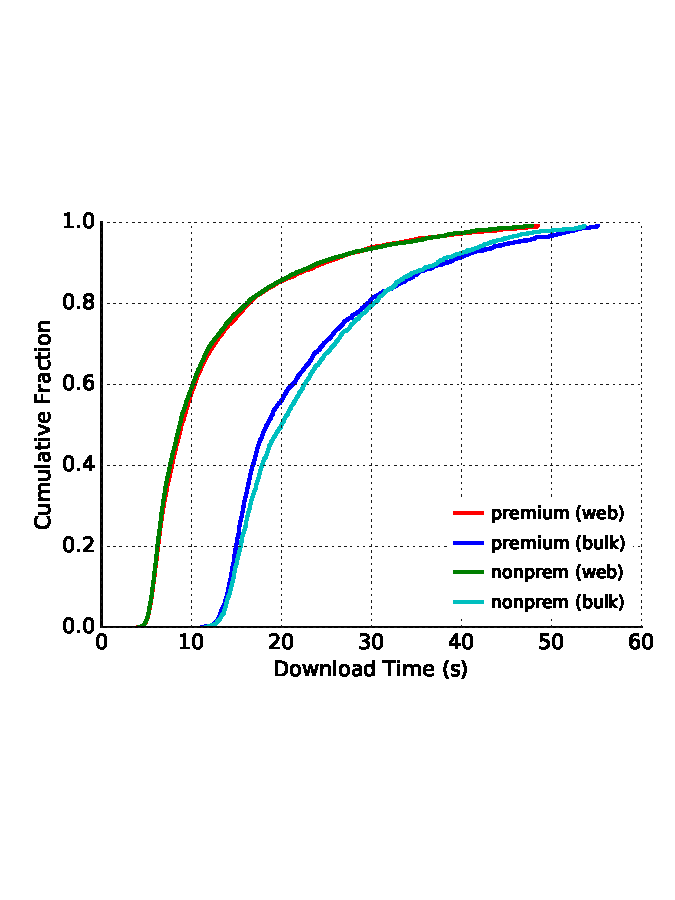
\includegraphics[trim={0 3cm 0 3cm}, clip,
    width=0.32\textwidth]{images/scheduling_priority.pdf}
  \caption[Prioritized Scheduling]{Prioritized Scheduling --- CDF download times
    for superimposed web and bulk clients where premium status is enforced only
    via scheduling. Almost no priority is observed.}
  \label{fig:scheduling_priority}
\end{figure}

\subsection{Investigation and discussion}

Our negative results indicate that scheduling is not the most decisive determining factor in performance.
To verify this hypothesis, we studied the incoming queue from which the scheduler can select new active circuits.
Figure~\ref{fig:scheduling_far} illustrates the temporal load in the queue at a single exit relay over one minute.
The height of the curve represents the total number of cells waiting to be serviced at each continuous point in time, while the colors group quantities of cells that belong to the same circuit.
Figure~\ref{fig:scheduling_close} displays a subset of the same information within a smaller time interval.\footnote{While the graph has the visual appearance of a bar graph, this is just a function of the striking data pattern.
In actuality, the plot displays a stacked area graph.}

In the figures mentioned earlier, notice that the queue is only populated for a period of 10 $ms$ before it is completely flushed, implying the queue spends the vast majority of its time empty.
This 10 $ms$ window is a product of Tor's internal event handling framework and is consistent with data from Jansen et al~\cite{jansen2018kist}.
We found in an analysis of the line-by-line observations of the queue activity that while cells get flushed in the correct order, they appear in the queue at roughly equal proportions.
In effect, bandwidth in our simulation is not constrained by the ordering policy of the scheduler but rather by the rate at which they arrive from the network.
As a consequence, local decisions at a particular relay for scheduling falls short of offering the expected priority.
Note that Jansen \textit{et al.}~\cite{jansen2018kist} discovered the same problem, which motivated the deployment of KIST.
Our results show that despite the use of KIST, relays may still be able to flush all queues at once, dismissing the effect of the scheduler's choice.

\begin{figure} \centering
  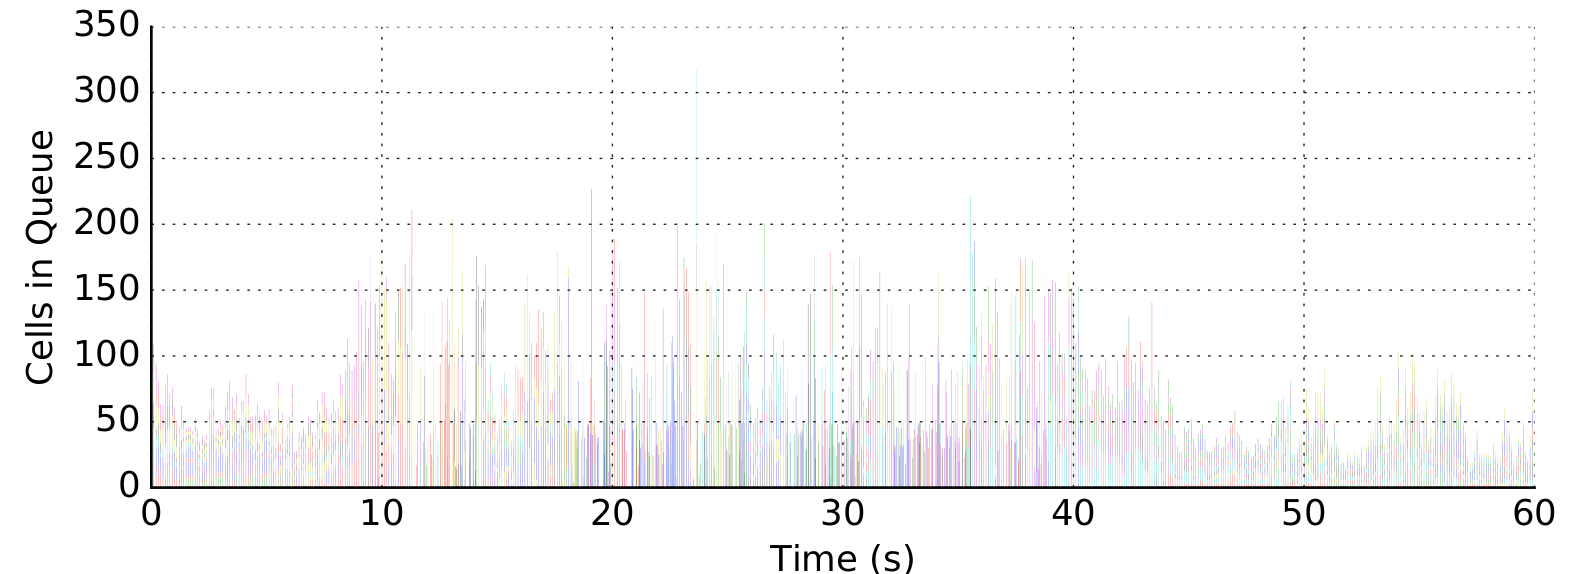
\includegraphics[width=0.49\textwidth]{images/scheduling_far.png}
  \caption[Queue Temporal Profile (60 seconds)]{Queue Temporal Profile (60
    seconds) --- Size of the scheduling buffer over time at a single exit relay
    in terms of number of cells. Colors group cells belonging to the same
    circuit.}
  \label{fig:scheduling_far}
\end{figure}

\begin{figure} \centering
  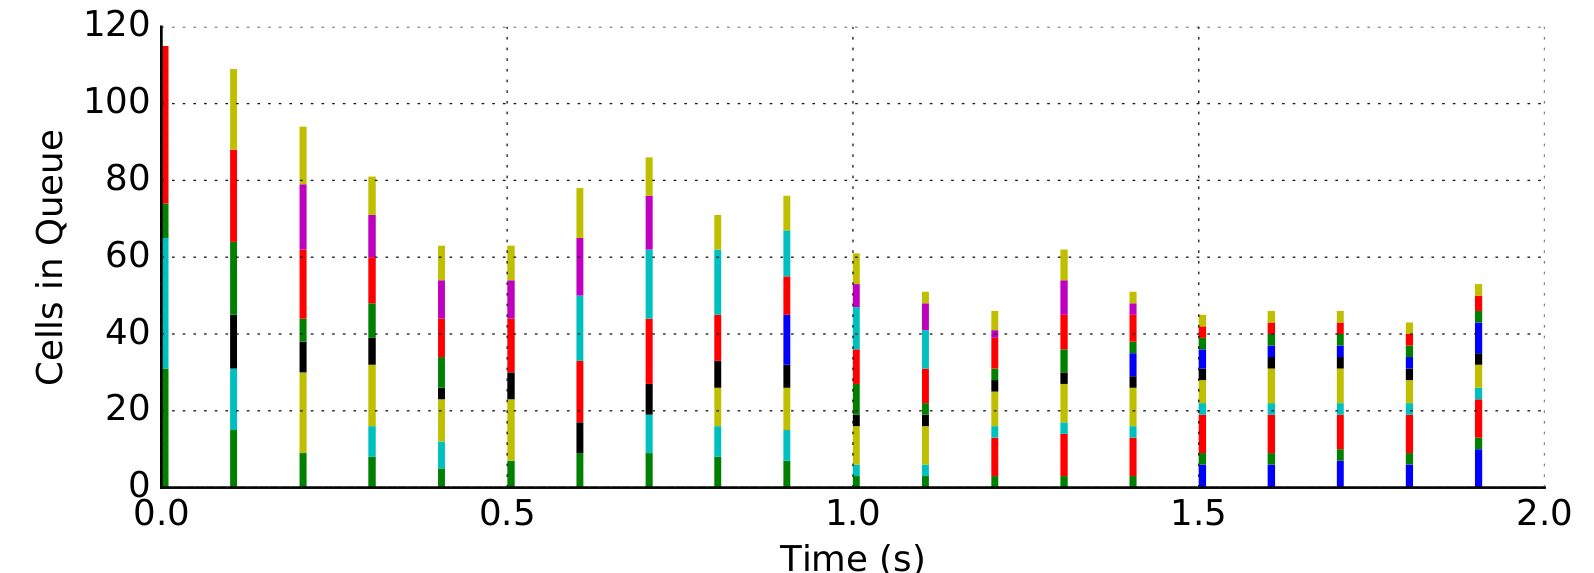
\includegraphics[width=0.49\textwidth]{images/scheduling_close.png}
  \caption[Queue Temporal Profile (2 seconds)]{Queue Temporal Profile (2
    seconds) --- Size of the scheduling buffer over time at a single exit relay
    in terms of number of cells. Colors group cells belonging to the same
    circuit.}
  \label{fig:scheduling_close}
\end{figure}


We now proceed to investigate why local relay scheduling does not work as expected.
Why do we fail to reproduce the positive results from previous works such as BRAIDS and LIRA despite using the same methodology?
First, it may be the case that other network control mechanisms within the Tor codebase constrain the flow of cells, rendering the mostly idle scheduler to be ineffective.
This could reflect any combination of factors including point-to-point flow control, connection throttling, or some less documented threshold embedded in the code.
However, we do not believe that the differences in the code explain fully explain our results.
As shown by our positive results in Section~\ref{sec:priority_exp}, the performance increases when we increase the circuit windows, a result which contradicts previous works exploring the effect of window sizes~\cite{archive-2009-mail, kiraly2008solving, dingledine2009performance}.
Moreover, the Tor code implementing these aspects did not meaningfully change over the years.
This information is likely linked to our failure to achieve prioritization via the scheduler.

To explain those oddities, we found and verified the following reason: the constraining network bottleneck has moved from the Tor network itself to the exit relay interface with external servers on the web.
In this scenario, cell queuing within Tor is not nearly as important as the TCP/IP packet handling at each exit relay.
Both approaches to prioritize flows are complementary: when the congestion is inside the Tor network, applying local scheduling policies makes an efficient priority mechanism, as demonstrated by previous works.
Also, in such a situation, priority based on the flow-control (that is, a function of the global circuit) would not be efficient because all cells would spend the majority of the time waiting in relays' FIFO queues.
Conversely, if the congestion is outside the Tor network (between the exit relays and the destination), then local scheduling policies would fall short of making any prioritization as showed in Figure~\ref{fig:scheduling_priority}.
Priority based on the flow-control would achieve to prioritize flows in this case, as demonstrated in Section~\ref{subsec:experiments}.

The shift of congestion from the internal Tor network to the exit gateways explains why our scheduling results in Figure~\ref{fig:scheduling_priority} are different from BRAIDS and LIRA.
Indeed, BRAIDS run experiments with Tor version \texttt{0.2.0.35} and a network history from January 2010~\cite{braids-repository}.
This Tor version's commit is before a major change in the path selection mechanism that reduced Tor's internal congestion problem and greatly improved the performance.
Mike Perry's commit \texttt{0ff86042ac16} affecting bandwidth weights introduced this major change in September 2010.
The bandwidth-weights are a set of weights specified in the directory specifications, section 3.8.4~\cite{dirspec}, that aim at balancing the overall network usage.
Those weights are critical for the network performance, and also for anonymity~\cite{waterfilling-pets2017, wf_proposal}.
Importantly, the benefit of Mike Perry's bandwidth-weights is proportional to the inequalities between the overall bandwidth in-circuit positions, which has grown rapidly over the years, as shown in Figure~\ref{fig:bw_inequalities}.

\begin{figure}
  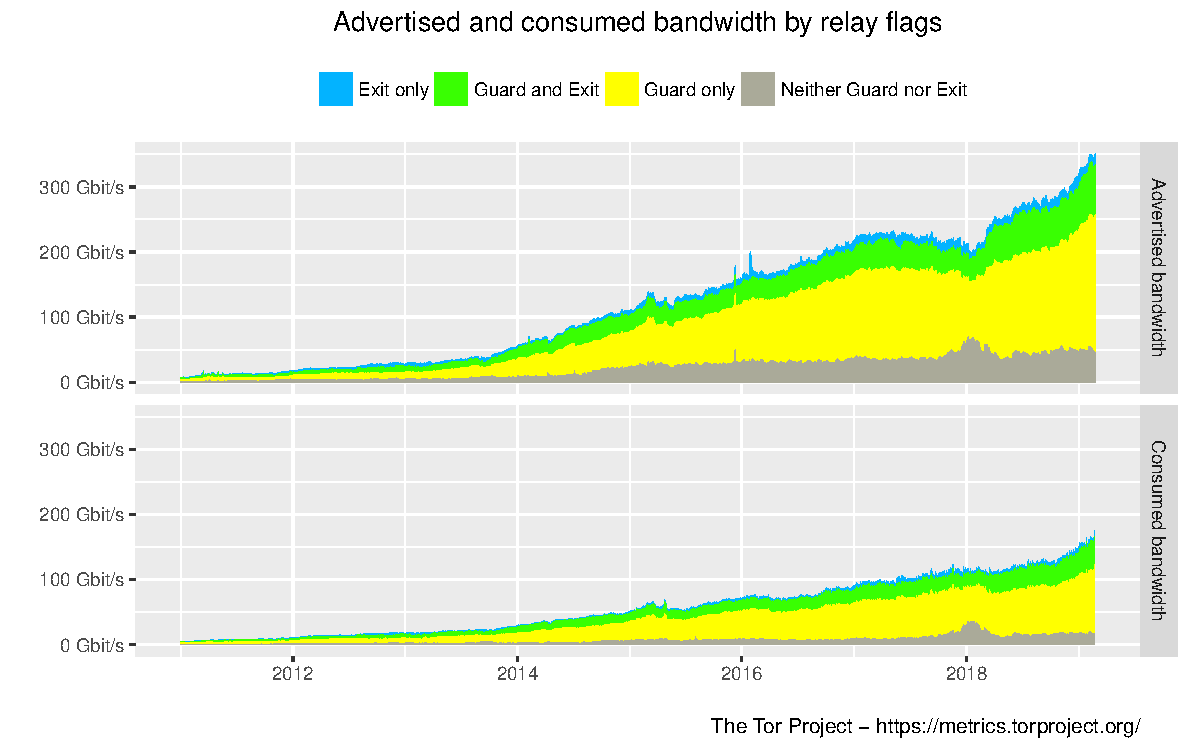
\includegraphics[scale=0.415]{images/bandwidth-flags-2011-01-01-2019-02-25.pdf}
  \caption{Evolution of bandwidth aggregated by relay flags.}
  \label{fig:bw_inequalities}
\end{figure}

LIRA's experiments ran on \texttt{tor-0.2.3.13-alpha} from March 2012, which benefits from Mike Perry's bandwidth-weights.
This timeline may explain why LIRA has less impressive priority advantage than the one exposed in BRAIDS.
Experiments in LIRA are probably less internally congested than the ones from BRAIDS, a change that is seemingly caused by the significant change in the path selection algorithm.
However, the different congestion status may also be due to other factors, such as a different client usage model and the local scheduling policies.
LIRA used a simulated environment scaled down from an April 2012 consensus where $\approx 42\%$ of relays had an \texttt{Exit} flag
Meanwhile, only $\approx 13\%$ of relays in our experiment had an \texttt{Exit} flag.
Figure~\ref{fig:bw_comp} plots the distribution of bandwidth allocated to each position and illustrates the different state of the Tor network, which in turn is reflected in the Shadow Simulations.
Consensus data in more recent years, which we use in moneTor's experiments, indicate network conditions where exit bandwidth is much scarcer~\cite{waterfilling-pets2017}.

\begin{figure}
	\centering 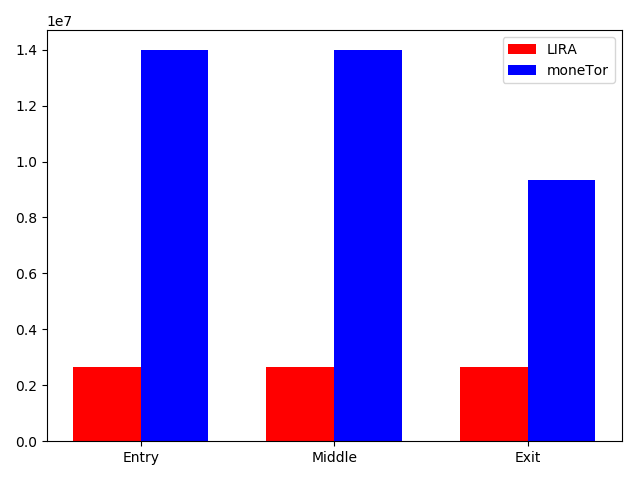
\includegraphics[scale=0.415]{images/bw_analysis_comp.png}
  \caption{Bandwidth distribution in consensuses used for BRAIDS, LIRA and moneTor experiments - BRAIDS does not benefit from bandwidth-weights to refill Middle, LIRA benefits from bandwidth-weights to offer balance between all positions, moneTor benefits from bandwidth-weights to balance entry and middle, yet does not have enough exit nodes to achieve the full balance}
  \label{fig:bw_comp}
\end{figure}
 
In summary, as the network grows to offer greater internal bandwidth (Figure~\ref{fig:bw_inequalities}, Figure~\ref{fig:bw_comp}), LIRA and BRAIDS's schedulers would tend to become less efficient for providing priority, as demonstrated in our experiments and showed in Figure~\ref{fig:scheduling_close}.
We should emphasize that this observation describes a coarse-grained trend.
Since our experiments ran on a scaled-down topology with simplistic models for user behavior, the results do not necessarily describe the state affairs for all relays in the real Tor network.
What can be said is that networking as a whole is an immensely complex and unpredictable domain and that the attainment of a simulation environment conducive to effective scheduling is, at the very least, nontrivial.
Any serious deployment of an incentivization scheme would require further research into robust prioritization mechanisms.
We leave this task for future work.
